% Preamble
\documentclass[11pt]{article}

% Packages
\usepackage{amsmath}
\usepackage{mathtools}
\usepackage{ragged2e}
\usepackage [utf8]{inputenc}
\usepackage{blindtext}
\usepackage{wrapfig}
\usepackage{xcolor}
\usepackage {polski}
\usepackage{multicol}
\usepackage[a4paper, total={5.7in, 8in}]{geometry}
\usepackage{graphicx}
\usepackage{amstex}
\usepackage{csvsimple}
\usepackage{changepage}
\usepackage{enumitem}
\usepackage[english]{babel}
\usepackage{biblatex}
\usepackage{caption}
\usepackage{indentfirst}
\usepackage{epstopdf-base}
\usepackage{textcomp}

% Document
\begin{document}
%    Nagłówek
    \begin{flushleft}
        Maciej Pierzchała 282 934 \hfill Data wykonania ćwiczenia:\\
        Filip Kubecki 272 655 \hfill 15 października 2024r\\
        \hfill Data sporządzenia sprawozdania:\\
        Grupa: Wtorek 10:35 \hfill 15 października 2024r\\
    \end{flushleft}
    \begin{center}
        \Large\textbf{Laboratorium 1}\\
        \textbf{Charakteryzacja czujników temperatury}
    \end{center}
    \hfill
%    Treść
    \section{Spis przyrządów}
    \par{
        Do wykonania ćwiczenia wykorzystano:
        \begin{itemize}
            \setlength\itemsep{0em}
            \item[-] Multimetr cyfrowy Sigilent SDM 3055
            \item[-] Termorezystor PT100
            \item[-] Termistor o nieznanych paramterach
            \item[-] Termopare o nieznanych parametrach
            \item[-] Pojemnik termiczny na gorącą wodę
            \item[-] Pojemnik z wymrożoną wodą
            \item[-] Blok metalu z otworami na sondy
        \end{itemize}
    }
    \section{Przebieg i cele doświadczenia}
    \noindent Doświadczenie polega na zmierzeniu wartości elektrycznych kolejnych przetworników:
    \begin{itemize}
        \setlength\itemsep{0em}
        \item[-] Termorezystora PT100 - rezytancja
        \item[-] Termistora - rezystancja
        \item[-] Termopary - napięcie
    \end{itemize}
    \par Jednocześnie wykonywano pomiar wartości na wszystkich 3 czujnikach. Pomiary obejmowały kolejno:
    \begin{itemize}
        \setlength\itemsep{0em}
        \item[-] Pomiar temperatury otoczenia
        \item[-] Pomiar temperatury wody z lodem (temperatura bliska 0\textdegree C)
        \item[-] Pomiar temperatury wrzącej wody
        \item[-] Pomiar temperatury stygnącej wody wykonywany w 5 min odstępach
    \end{itemize}
    
    \section{Obliczenia i analiza wyników}
    \subsection{Termorezystor PT100}
    TWR wyznaczono z zamieszczonego niżej wzoru:
    \begin{gather*}
        TWR=\frac{(R_2-R_1)\cdot 10^6}{R_1(T_2-T_1)}\quad [ppm/K]
    \end{gather*}
    \indent Gdzie:
        {\footnotesize
    \begin{itemize}
        \setlength\itemsep{0em}
        \item[] \textbf{$R_1$} - rezystancja w temperaturze $T_1$
        \item[] \textbf{$R_2$} - rezystancja w temperaturze $T_2$
    \end{itemize}}
    Dla $T_1$ równego $0^{\circ}$C, oraz $T_2$ równego $100^{\circ}$C:
    \begin{gather*}
        TWR=\frac{(138.503\Omega-100.08\Omega)\cdot 10^6}{100.08\Omega\cdot(100^{\circ} C-0^{\circ}C)}=\frac{(38.423\Omega)\cdot 10^6}{100.08\Omega\cdot(100^{\circ}C)}=3839.2286\dots[ppm/K]
    \end{gather*}
    \indent Przekształcając powyższy wzór oraz wykorzystując wyliczoną wartość TWR możemy wyznaczyć temperaturę mierzoną termorezystorem na podstawie zmierzonej rezystancji:
    \setlength{\jot}{10}
    \begin{gather*}
        TWR=\frac{(R_2-R_1)\cdot 10^6}{R_1(T_2-T_1)} \\
        TWR\cdot R_1=\frac{(R_2-R_1)\cdot 10^6}{T_2-T_1} \\
        \frac{TWR\cdot R_1}{(R_2-R-1)\cdot 10^6}=\frac{1}{T_2-T_1} \\
        T_2-T_1=\frac{(R_2-R_1)\cdot 10^6}{TWR\cdot R_1}\\
        T_2=\frac{(R_2-R_1)\cdot 10^6}{TWR\cdot R_1}+T_1
    \end{gather*}
    Podstawiając wartości stałe:
    \begin{gather*}
        T_2=\frac{(R_2-100.08)\cdot 10^6}{3839.2286\cdot 100.08}
    \end{gather*}
    Przykładowo dla drugiego pomiaru studzenia się wrzątku:
    \begin{gather*}
        T_2=\frac{(131.88-100.08)\cdot 10^6}{3839.2286\cdot 100.08}=\frac{31.8\cdot 10^6}{384229.9982}=82.7629^{\circ}C
    \end{gather*}
    \newpage
    Na przy pomocy powyższego wzóru wyznaczono temperaturę wszystkich punktów stygnięcia wody oraz wyznaczono charakterystykę
    rezystancji od temperatury:\\
    \noindent\makebox[\textwidth]{
        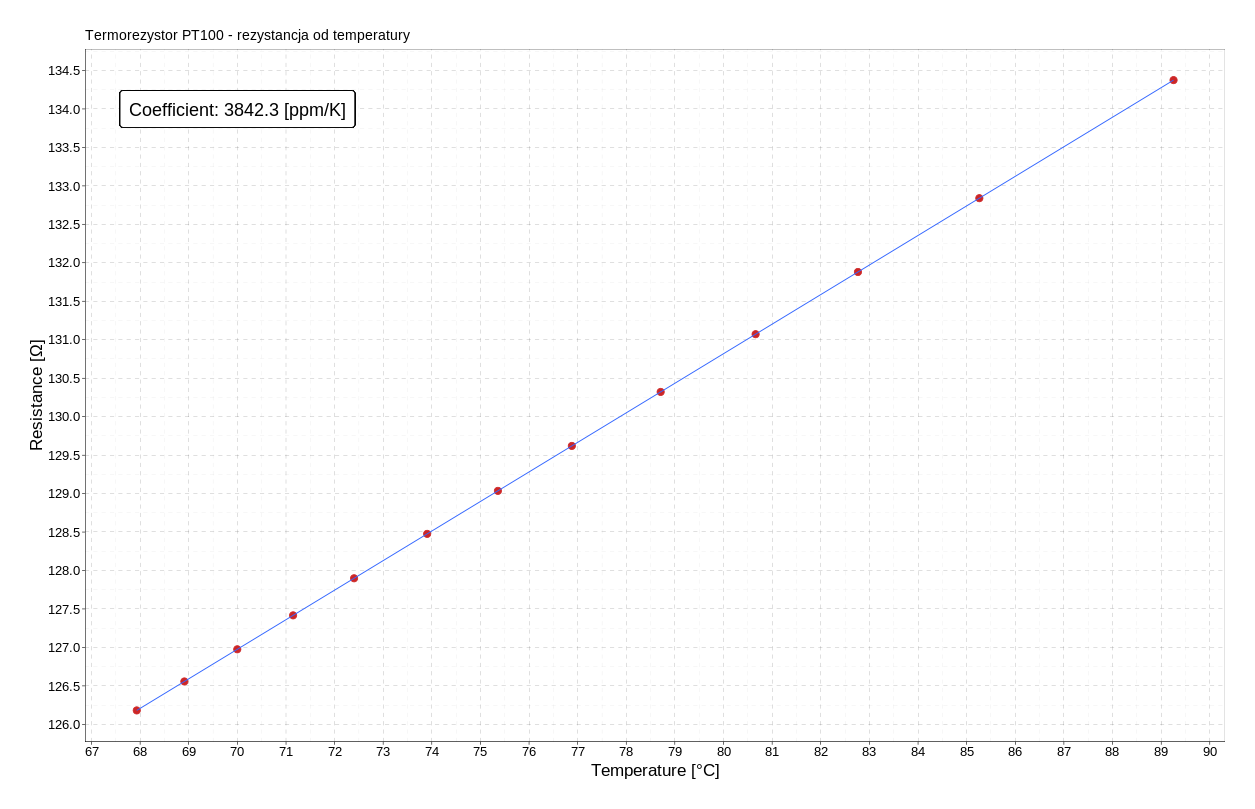
\includegraphics[scale = 0.46]{/home/bork/IdeaProjects/LatexProjects/src/PodstawyTechnikiSensorowej/Lab1/Img/pt100.png}
    }
    \indent Możemy zauważyć ze współczynni kierunkowy funkcji który został podany na wykresie jest bardzo zbliżony do wartości obliczonej z wzoru. Niewielka
    różnica wynika jedynie z tego, iż we wzorze na temperaturę na podstawie rezystancji wykorzystano jako referencje rezystancję w 0 stopni, która odbiega
    minimalnie od wartości poprawnej.\\
    \indent Również funkcja tworząca model liniowy który wyznaczył wspłczynnik kierunkowy z regresji liniowej mógł wprowadzić
    niewielkie zmiany wynikające z dokłądności każdego pomiaru.
    \newpage
    \subsection{Termistor}
    \par Stworzono charakterystykę rezystancji od temperatury dla naszego termistora o niewiadomych parametrach:\\
    \noindent\makebox[\textwidth]{
        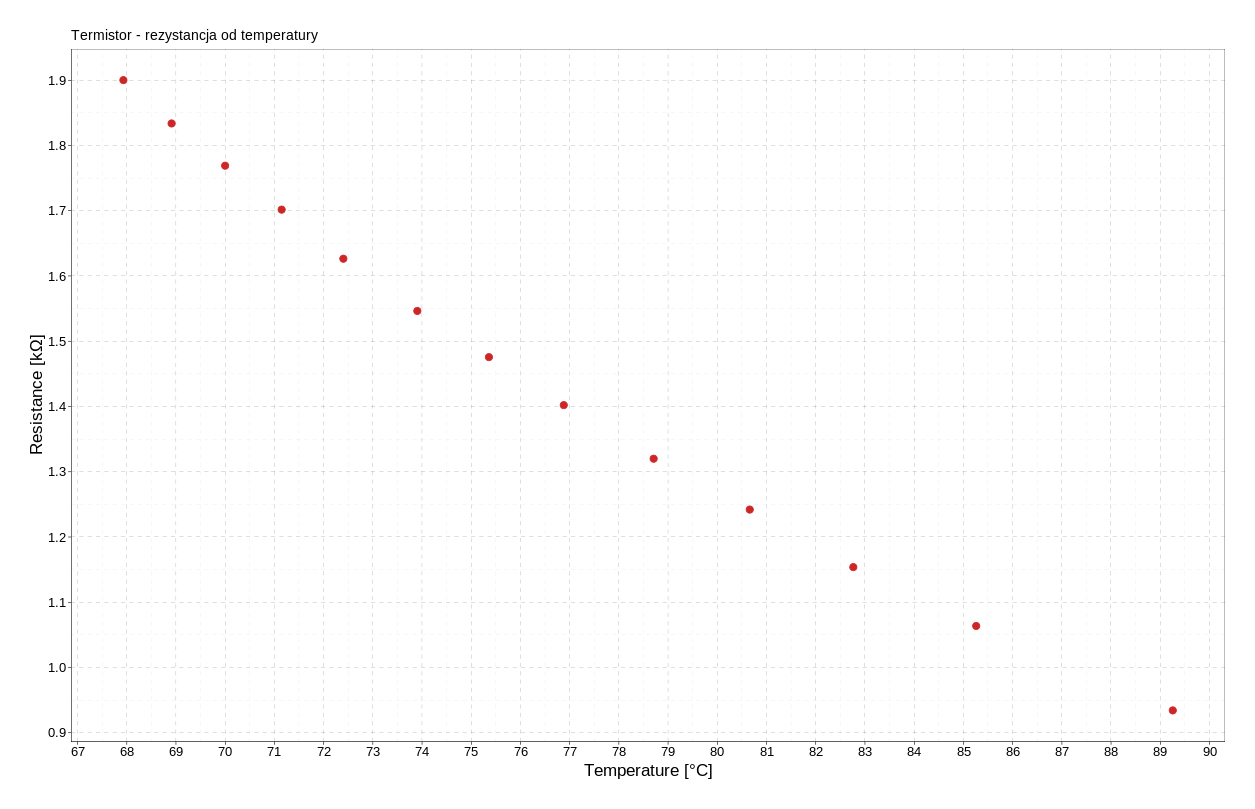
\includegraphics[scale = 0.46]{/home/bork/IdeaProjects/LatexProjects/src/PodstawyTechnikiSensorowej/Lab1/Img/thermistor.png}
    }
    \indent Na podstawie charakterystyki jesteśmy w stanie określić że badany termistor to termistor
    typu \textbf{NTC} (ang. \textit{\textbf{N}egative \textbf{T}emperature \textbf{C}eoefficient}). Wynika to z tego że wraz ze wzrostem temperatury
    rezystancja termistora spada.\\
    \indent Następnie wyznaczono charakterystykę $ln\frac{R_t}{R_0}=f(\frac{1}{T}-\frac{1}{T_0})$. Współczynnik kierunkowy tej charakterystyki
    wyznaczy nam współczynnik materiałowy termistora \textbf{$\beta$}.\\
    \indent Współczynnik kierunkowy funkcji wyliczony przy użyciu regresji liniowej wynosi w zaokrągleniu  $4096.032 [K]$. Na kolejnej stronie
    przedstawiono wykres chrakterystyki na której podstawie wyliczono współczynnik materiałowy.
    \newpage
    \noindent\makebox[\textwidth]{
        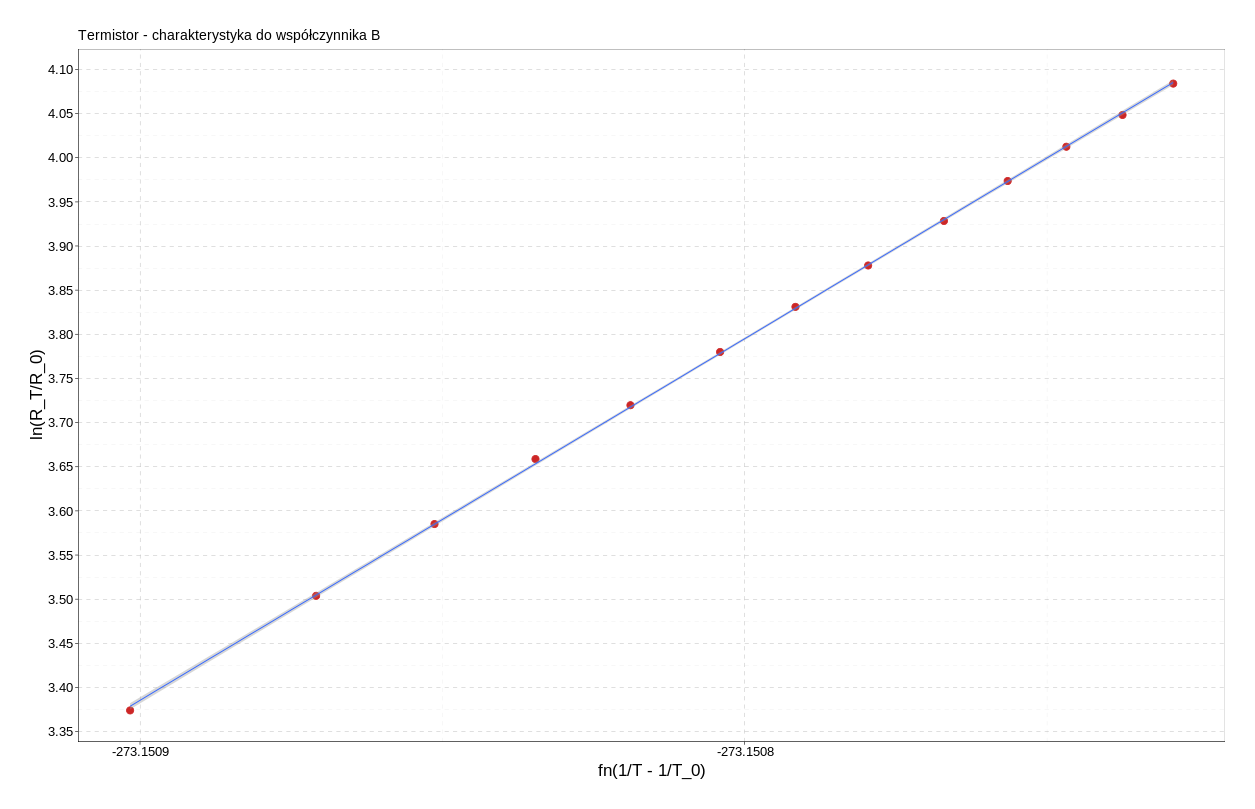
\includegraphics[scale = 0.46]{/home/bork/IdeaProjects/LatexProjects/src/PodstawyTechnikiSensorowej/Lab1/Img/termistorB.png}
    }
    \indent Korzystając z wyznaczonego współczynnika materiałowego oraz rezystancji w temperaturze pokojowej możemy wnioskować że jest to termistor o rezystancji 10 [k$\Omega$] typu NTC
    oraz o stałej materiałowej w przedziale od 4000 do 4200 [K]. Przykładowe termistory o podobnych parametrach:
    \begin{itemize}
        \item[-] NTCM-10K-B4150 firmy SR PASSIVES
        \item[-] NTCC-10K firmy SR PASSIVES
        \item[-] NTC 10k firmy ESCO
        \item[-] Thermistor NTC 10K 5\% B4100 (MF52A103J4100)
    \end{itemize}
    \newpage
    \subsection{Termopara}
    \par Na podstawie wcześniej wyznaczonych danych oraz pomiarów wyznaczono charakterystykę napięcia od temperatury dla termopary:\\
    \noindent\makebox[\textwidth]{
        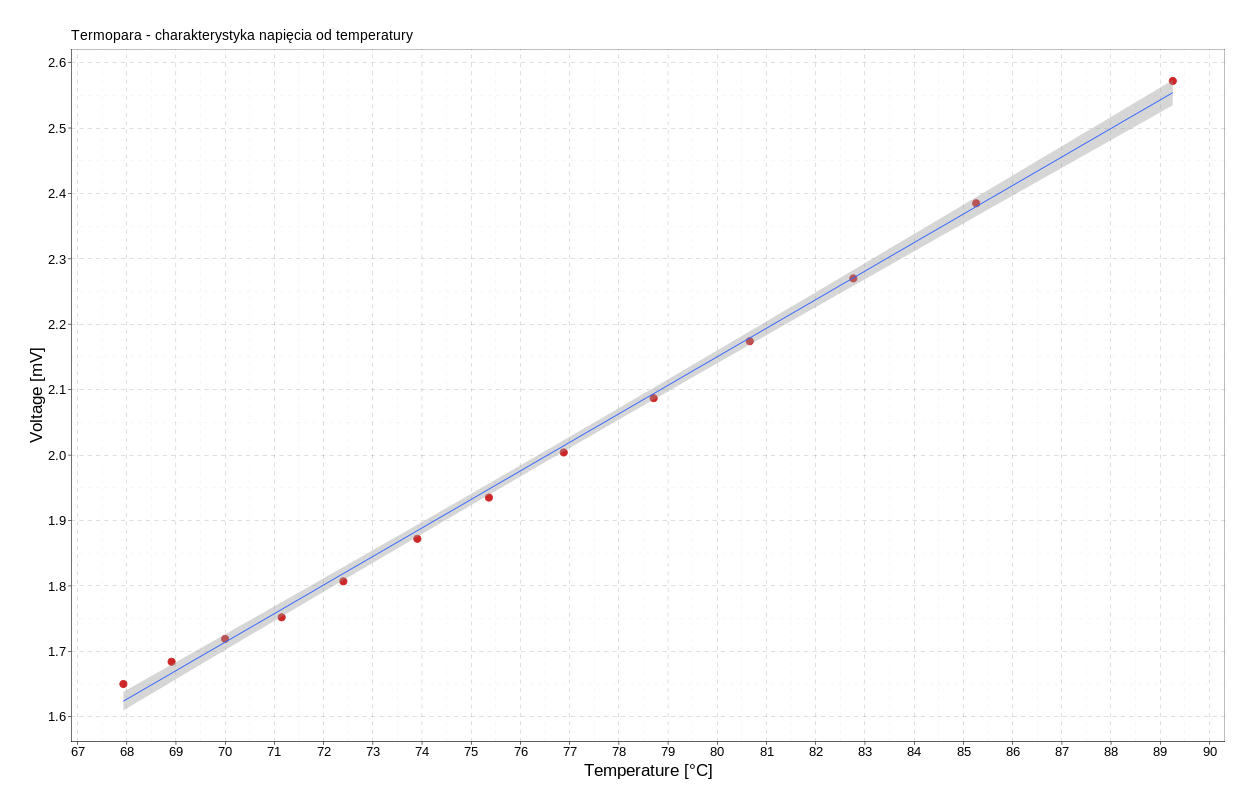
\includegraphics[scale = 0.46]{/home/bork/IdeaProjects/LatexProjects/src/PodstawyTechnikiSensorowej/Lab1/Img/thermalCouple.png}
    }
    \indent Jednocześnie na wykresie przedstawiono regresję liniową dla podanych punktów. Zrobiono to aby wyznaczyć na podstawie regresji
    współczynnik Seebecka. Nie tworzono kolejnego wykresu dla zależności $\varepsilon_m=f(T_2-T_2)$ gdyż zmiany które występują w przedstawionej
    funkcji jedynie przesuwają funkcję w układzie współrzędnych ale nie zmieniają kąta nachylenia funkcji. Współczynnik kierunkowy więc dla tej chrakterystyki
    oraz dla wykresu powyżej będą identyczne.\\
    \indent Współczynnik Seebecka wyznaczony z regresji liniowej wynosi $43.62[\mu V/K]$. Na podstawie wyników jesteśmy w stanie stwierdzić
    iż pracowaliśmy z termoparą typu K (można poznać bo kolorach wyprowadzeń które są koloru białego i zielonego) ze spoiną zrobioną z
    połączenia chromelu i alumelu. Spoina taka posiada współczynnik Seebecka o wartości około 40 [$\mu V/K$].

    \section{Wnioski}
    \par Dla termorezystora PT100 wartości rezystancji zmieniają się liniowo wraz ze wzrostem temperatury
    co jest z godne z charakterystyką tego typu czujnika. Obliczony współczynnik temperaturowy rezystancji (TWR)
    wyniósł 3839,23 ppm/K, co dobrze odzwierciedla zmianę rezystancji w zakresie temperatur od 0°C do 100°C.
    Różnice między obliczoną a zmierzoną temperaturą wynikają z drobnych błędów pomiarowych oraz założeń dotyczących
    rezystancji w temperaturze 0°C.
    \\

    \indent Termistor wykazał spadek rezystancji wraz ze wzrostem temperatury, co potwierdza, że był to termistor typu NTC.
    Na podstawie charakterystyki oraz obliczeń współczynnika materiałowego (β ≈ 4096 K), stwierdzono, że termistor ma
    rezystancję nominalną 10 kΩ. Parametry termistora są zbliżone do popularnych modeli, takich jak NTCM-10K-B4150 czy NTC 10k.
    \\

    \indent Charakterystyka napięcia w funkcji temperatury dla termopary wykazała liniową zależność, z wyznaczonym współczynnikiem
    Seebecka na poziomie 43,62 µV/K.\\
    \indent Na podstawie charakterystyki napięciowej oraz kolorów przewodów, zidentyfikowano termoparę jako typ K, której współczynnik
    Seebecka wynosi około 40 µV/K.
    %Bibliografia
    \vfill
    \footnotesize
    \begin{thebibliography}{3}
        \bibitem{texbook1}
        https://en.wikipedia.org/wiki/Seebeck\_coefficient
        \bibitem{texbook2}
        https://pl.wikipedia.org/wiki/Temperaturowy\_współczynnik\_rezystancji
        \bibitem{texbook3}
        https://en.wikipedia.org/wiki/Thermistor
        \bibitem{texbook4}
        https://www.tme.eu/pl/details/ntcm-10k-b4150/termistory-ntc-pomiarowe-tht/sr-passives/

    \end{thebibliography}
\end{document}